\documentclass{scrartcl}[12pt,a4paper]
%\documentclass{article}[12pt,a4paper]
%\documentclass{artikel3}[12pt,a4paper]

\usepackage{minted}
\usepackage{hyperref}
\usepackage{graphicx}
\usepackage{xcolor}
\usepackage{cmbright}
\usepackage[T1]{fontenc}

\begin{document}

\title{Tutorial for the MOONS FPU grid driver Python library
  module} \subtitle{For driver version 0.5.0 (document version \texttt{\input{../git_version}})}

\author{Johannes Nix}

\maketitle

\tableofcontents


\section{Introduction}
\subsection{Topic and goals}
This tutorial describes how to use the Python bindings for the MOONS
fibre positioner unit (FPU) driver. Its goal is to enable the reader
to control the FPU in the verification system using python scripts, so
that he or she can perform basic verification tasks.


\subsection{Required knowledge}

It is assumed that the reader has basic knowledge of Python, or,
alternatively, a similar object-oriented language, like Java or C\#.
In the case that using Python scripts is new to the reader, it is
probably helpful to consult the tutorial for Python 2.7 at
\url{https://docs.python.org/2.7/tutorial/}.  Both the current version
of the driver as well as this document use Python 2.7. Python 2 has
some differences to Python 3. However this description will proceed in
a way that differences to Python 3 are minimised.

Also, in order to retrieve the current version of the library, the
user needs to have a minimum knowledge of the git version control
system. This is explained, for example, in
``\href{https://git-scm.com/book/en/v2/Git-Basics-Getting-a-Git-Repository}{getting
  a git repository}''.

\section{Setting up the library module}

\subsection{Getting the source code}

To set up the library module, it is first
necessary to retrieve a current copy of its source code.
On the moons-pc01 workstation, this can be done using the
command \mint{bash}|git clone /home/jnix/fpu_driver|
This creates a new directory with the name \texttt{fpu\_driver}
and populates it with the source code.

Alternatively, a fresh copy can be retrieved from the UKATC dalriada
server. Doing this this requires a personal user account on that
server. Assuming the account name is \texttt{carl}, this is done by
the command

\mint{bash}|git clone carl@dalriada/sw/sw4/jnix/MOONS/fpu_driver|

After entering the password for user \texttt{carl}, the
source code is copied into the new folder \texttt{fpu\_driver}.

\subsection{Refreshing the source code}
To refresh the source code, change the
working directory to \texttt{fpu\_driver},
and issue the command

\mint{bash}|git pull|


\subsection{Building specific revisions}
In the default case, the library is build from
the master branch of the git repository.
The master branch contains the most current
working version.
In some cases, it might be required to
use a specific revision of the library.
Assuming that we need, as an example,
to build version v0.5.2 of the library,
checking out this revision is done with the
command

\mint{bash}|git checkout v0.5.2|

After this, one can proceed with building the library as normal. To
switch back to the master branch, issue the command

\mint{bash}|git checkout master|


\subsection{Building the library module}

To build the Python library module,
change the working directory to \texttt{fpu\_driver},
and issue the command \mint{bash}|make pyext|

In order for this to work, the required dependencies need to be
installed. For the MOONS workstation, this is always the case. To
install these dependencies on other computers, follow the detailed
instructions in the file ``\texttt{doc/INSTALL}''.

\subsection{Environment configuration}

For the Python module to work, the directory \texttt{/user/local/lib}
needs to be added to the environment variable
\texttt{LD\_LIBRARY\_PATH}.  Assuming a standard setup, this can be
done by adding the following line to the file \texttt{.bashrc} in the
user-specific home directory:

\begin{minted}{bash}
  export LD_LIBRARY_PATH=$LD_LIBRARY_PATH:/usr/local/lib
\end{minted}

All the examples presented here assume that the current working
directory is \texttt{fpu\_driver/python}. If this is not the case,
this directory needs to be added to the \texttt{PYTHONPATH}
environment variable.


\subsection{Communication protocol versions}

The FPU driver sends commands to the fibre positioner units, which use
a specific communication protocol. This protocol needs to match the
FPUs firmware and its capabilities. The current version of the driver
(version 0.5.0) uses ``communication protocol version 1'', which has
some restrictions in functionality. For example, some edge cases
cannot be checked, some operations might take longer, and some errors
are not recognised or cannot as easily worked around.

There are two significant differences which are visible to the users
of the FPU driver module. Both need careful consideration.

The first is that is that cases in which the alpha arm of the FPU hits
the limit switch need to be manually recovered from. This is explained
in section~\ref{sec:recovery} on page~\pageref{sec:recovery}.

Second, the \texttt{findDatum()} command mandatory requires that,
before starting the datum search, \textbf{the beta arm is in a
  counter-clockwise position relative to the datum switch}. If the
the step counters have valid values, it needs to be in a positive
range of valid step counts from the datum switch, or at count zero. If
the beta arm has a position corresponding to the negative range (that
is, clock-wise from the datum position), it needs to be manually moved
first.  This applies also when the step counters in the meantime have
been invalidated by a \texttt{resetFPU()} command or by powering off the
FPU.


\section{A minimal example}
\label{sec:minimalexample}
The following listing shows a minimal example of the
driver usage, and explains the underlying concepts
step by step.

\begin{minted}[linenos]{python}

from __future__ import print_function
import FpuGridDriver
from FpuGridDriver import TEST_GATEWAY_ADRESS_LIST
from fpu_commands import list_positions, list_angles, \
       list_deviations, list_states, gen_wf
# print the driver version, just to check
print("The FPU driver version is:", FpuGridDriver.__version__,
      ", CAN PROTOCOL version:", FpuGridDriver.CAN_PROTOCOL_VERSION)

NUM_FPUS = 1
gd = FpuGridDriver.GridDriver(NUM_FPUS)

print("connecting grid:", gd.connect(address_list=TEST_GATEWAY_ADRESS_LIST))

print("getting grid state:")
grid_state = gd.getGridState()


print("issuing findDatum:")
gd.findDatum(grid_state)
print("findDatum finished")

# We use grid_state to display the starting position
print("the starting position (in degrees) is:", list_angles(grid_state))


# Generate a waveform which moves the alpha arm by +45
# degree, and the beta arm by +15 degree. 

alpha_move = 45
beta_move = 15

# Generate the required waveform for one FPU
waveform = gen_wf(alpha_move, beta_move)

# upload the waveform to the FPU
gd.configMotion(waveform, grid_state)

# start the movement
print("starting movement by (45,15) degree")
gd.executeMotion(grid_state)

print("the reached position (in degrees) is:", list_angles(grid_state))

print("ready")

\end{minted}


\subsection{Import statements}

The import statements in lines 1 -- 4 load the following modules and
configurations:

\begin{itemize}
\item In line 1, the print function and the division operator is
  configured to work as in Python 3.
  
\item ``\texttt{import FpuGridDriver}'' in line 2 loads the driver
  library module. (If this import command fails, check that both
  \verb+LD_LIBRARY_PATH+ and \verb+PYTHONPATH+ have the right values.)

\item The line ``\texttt{from FpuGridDriver import
  TEST\_GATEWAY\_ADRESS\_LIST}'' loads a default address which refers to
  the EtherCAN gateway which is used. This address will be different
  when one wants to select a different gateway.

\item The line ``\texttt{from fpu\_commands import \ldots}'' imports a
  few utility commands which help to display positions and to generate
  movement waveforms.

 
\end{itemize}

\subsection{Grid driver object}

In line 10, the used number of FPUs is set to one, and in line 11, the
FPU grid driver is initialised with that value. The returned object,
which is referenced by the Python variable \texttt{gd}, is always
required to access the FPUs.

\subsection{Driver methods}

The driver object allows to invoke method calls (methods are also
often called member functions) which control the FPU hardware. The
method names always start with a dot after the name of the driver
object.  So, \texttt{gd.abc()} would call method ``abc'' of the driver
object. Like normal function calls, they usually have parameters.

In this case, the method \texttt{connect()} connects the driver to one
or more EtherCAN gateways and starts listening to messages from the
FPUs. The parameter defines to \emph{which} gateways the driver
listens to.

As can be seen in the example, the methods have return values.  In
case of serious errors, the methods raise a Python exception. The
Python program does not need to explicitly disconnect and
de-initialise the driver, this happens automatically when the program
terminates\footnote{However if required, you can use the statements
  \texttt{gd.disconnect()} and \texttt{del gd}, which disconnects and
  deletes the driver object.}.



\subsection{Grid state variable}

Almost all commands to the driver receive and return a snapshot of the
current state of the used FPU (or, if there are several, of all of
them). That snapshot is passed in a variable called
\texttt{grid\_state}. This variable contains all the information a
user might need about the state of the FPUs - their current positions,
which commands they will accept, whether there are any collisions,
whether the step counters have been zeroed, whether a limit switch was
hit, and so on. With each invocation of a method, the old grid state
is passed as a reference parameter, and its new value is returned in
the same variable.

To retrieve a current grid state information, the method
``getGridState()'' is used, as is done in line 16. In our listing, the
grid state variable is assigned to the variable \texttt{grid\_state}.
The \texttt{getGridState()} function always returns immediately, as it
just takes a snapshot. Because \texttt{grid\_state} is used so
frequently, a short-hand name which many of the example scripts use is
the name \texttt{gs}.

\subsection{Moving the FPU around}

The example script then proceeds to use three methods to move
the FPUs:

\begin{description}
\item[\texttt{findDatum()}] in line 20 moves the FPU to the datum
  position. After this, the internal step counters are set to zero,
  both for the alpha and for the beta arm.

\item[\texttt{configMotion()}] is a method which sends a table with movement
  operations, also called waveform table, to the FPU. In the listing,
  this is done in line 37. The movement table is stored in the
  variable \texttt{waveform}, which is defined in line 34.

\item[\texttt{executeMotion()}] in line 41 is the command which starts
  the movement of the FPU. This command returns when the movement is
  complete and the FPUs have stopped to move. In case of an error, the
  command generates a Python exception.

\end{description}

\subsection{Utility functions}

The example also shows two utility functions for generating movement
data, and displaying information about the FPU state:

\begin{description}
\item[\texttt{list\_angles()}] is a function which takes a \texttt{grid\_state}
  variable, and displays the approximate positions of the FPUs as
  alpha and beta angles, in degree units.

\item[\texttt{gen\_wf()}] is a function which takes an (alpha,beta)
  pair of angle values, scaled in degrees, and generates a valid
  waveform which can be send to the FPU.  The waveform which is passed
  is a regular Python data structure and can be displayed and
  manipulated like any other Python object.  The user only needs to
  tale care that it contains valid movement data when it is passed to
  the \texttt{configMotion()} method!

\end{description}

\subsection{Interactive inspection of the FPU state}

\label{sec:fpustate}
The grid state variable holds a large amount of detail information
about the current state of FPUs. This is by design, because upper
layers of the software need to be able to deal with errors such as
collisions, and correct them. However, only a part of this information
is required by the verification system.

When trying to diagnose and understand errors, it is often helpful to
access this state information in an interactive way.  To do this, we
can make use of the capability that Python can run any commands which
appear in a script equally well when entered interactively. Also, the
Python interpreter can be started with the ``-i'' (interactive) option
which has the effect that after an exception, or after all commands in
a script have been executed, the interpreter opens a command line or
``read-eval-print-loop'' in which commands can be entered and executed
in the interactive mode. Every time when a typed-in expression or
function call returns a value, the value is printed out before the
command prompt appears again.

For example, let's assume that the script on
page~\pageref{sec:minimalexample} is shortened to the first 36 lines
and stored to a file named \texttt{short\_script.py}. We then might
run the following interactive session (where the lines starting with
``\texttt{\$}'' and ``\verb+>>>+'' are interactive input, and
everything else is output):



\begin{minted}{python}

  
$ python -i short_script.py
initializing driver:  DE_OK
connecting grid: DE_OK
getting grid state:
issuing findDatum:
findDatum finished
the starting position (in degrees) is: [(0.0, 0.0)]
>>> grid_state.FPU[0]
{ 'last_updated' : 61547082.491 'pending_command_set' : 0
  'pending_command_set' : 0 'state' : 'READY_FORWARD'
  'last_command' : 1 'last_status' : 0 'alpha_steps' : 0
  'beta_steps' : 0 'alpha_deviation' : 0 'beta_deviation' : 0
  'timeout_count' : 0 'step_timing_errcount' : 0
  'direction_alpha' : 0 'direction_beta' : 0
  'num_waveform_segments' : 0 'num_active_timeouts' : 0
  'sequence_number' : 0 'ping_ok' : 0 'movement_complete' : 0
  'was_zeroed' : 1 'is_locked' : 0 'alpha_datum_switch_active' : 0
  'beta_datum_switch_active' : 0 'at_alpha_limit' : 0
  'beta_collision' : 0 'waveform_valid' : 1 'waveform_ready' : 1
  'waveform_reversed' : 0 }
>>> list_angles(grid_state)
[(0.0, 0.0)]
>>> gd.executeMotion(grid_state)
fpu_driver.E_DriverErrCode.DE_OK
>>> grid_state.FPU[0]
{ 'last_updated' : 61547154.98 'pending_command_set' : 0
  'pending_command_set' : 0 'state' : 'RESTING'
  'last_command' : 7 'last_status' : 0 'alpha_steps' : 5625
  'beta_steps' : 1200 'alpha_deviation' : 0 'beta_deviation' : 0
  'timeout_count' : 0 'step_timing_errcount' : 0
  'direction_alpha' : 0 'direction_beta' : 0
  'num_waveform_segments' : 0 'num_active_timeouts' : 0
  'sequence_number' : 0 'ping_ok' : 1 'movement_complete' : 1
  'was_zeroed' : 1 'is_locked' : 0 'alpha_datum_switch_active' : 0
  'beta_datum_switch_active' : 0 'at_alpha_limit' : 0
  'beta_collision' : 0 'waveform_valid' : 1 'waveform_ready' : 0
  'waveform_reversed' : 0 }
>>> list_angles(grid_state)
[(45.0, 15.0)]
>>>
\end{minted}

In this listing, \verb+grid_state.FPU[0]+ displays the state parameters of
FPU 0 (which is the only one we have because \texttt{NUM\_FPUS} was
set to 1).

Just to pin-point two of the more important bits of information, the
fields ``alpha\_steps'' and ``beta\_steps'' contain the current step
counts of an FPU, and the fields 'alpha\_datum\_switch\_active' and
'beta\_datum\_switch\_active' contain the current position of the
datum switches. The field \texttt{state} contains the current state of
the FPU. One can see that after issuing the \texttt{executeMotion}
command, the state of the FPU changes from \texttt{READY\_FORWARD} to
\texttt{RESTING}. Actually, the output of the \texttt{list\_angles()}
utility function is just a scaled version of the ``alpha\_steps'' and
``beta\_steps'' fields. The flag \texttt{was\_zeroed} is set to
\texttt{True} when the datum position was reached at least once since
the driver was started, and no collisions, limit switch breaches, or
abortMotion commands have happened since.

\subsection{FPU states}
The state of an FPU is summarised in a enumeration value, which is
stored in the attribute \texttt{state}. For example, the state of FPU 0
can be retrieved by

\begin{minted}{python}

>>> grid_state.FPU[0].state
\end{minted}


\begin{table}
  \begin{centering}
\begin{tabular}{|l|p{0.6\textwidth}|}
  \hline
  \textbf{State name} & \textbf{Description} \\
  \hline 
UNKNOWN & The state of the FPU is not known, the driver needs to
be connected to the EtherCAN gateway first and retrieve the state.\\
\hline
UNINITIALIZED & The FPU has been pinged successfully, but it was
  so far not zeroed to the datum position, so no movements are
  possible.\\
\hline
LOCKED & The FPU was locked, which inhibits movement of this
  FPU.\footnote{This is a facility provided by protocol version 2}\\
\hline
DATUM\_SEARCH & The FPU is currently searching for the datum
position.\\
\hline
AT\_DATUM      & The FPU has reached the datum position.\\
\hline
LOADING & The FPU is currently configuring a new movement waveform.\\
\hline
READY\_FORWARD & The FPU is ready to move in the forward
  direction of the waveform table.\\
\hline
READY\_BACKWARD& The FPU is ready to move backwards along the
  waveform table.\\
\hline
MOVING        & The FPU is currently moving.\\
\hline
RESTING       & The FPU has finished its movement.\\
\hline
ABORTED & The movement was aborted, either by an internal error,
  or by an explicit abortMotion command.\\
\hline
OBSTACLE\_ERROR& The FPU has either detected a collision of the
  beta arm, or the alpha arm has hit the limit switch. In both cases, the
  movement was aborted. \\
\hline
\end{tabular}
\end{centering}
\caption{List of FPU states and their definitions}
\label{tab:fpustates}
\end{table}


Generally, each FPU is always in one of 12 different states.Each state
allows different commands, and commands can change the FPU state.
Some of the states are visited during any normal operation of the FPU,
and some are reached as a result of errors.  Table~\ref{tab:fpustates}
on page~\pageref{tab:fpustates} lists the different states.

\begin{figure}

  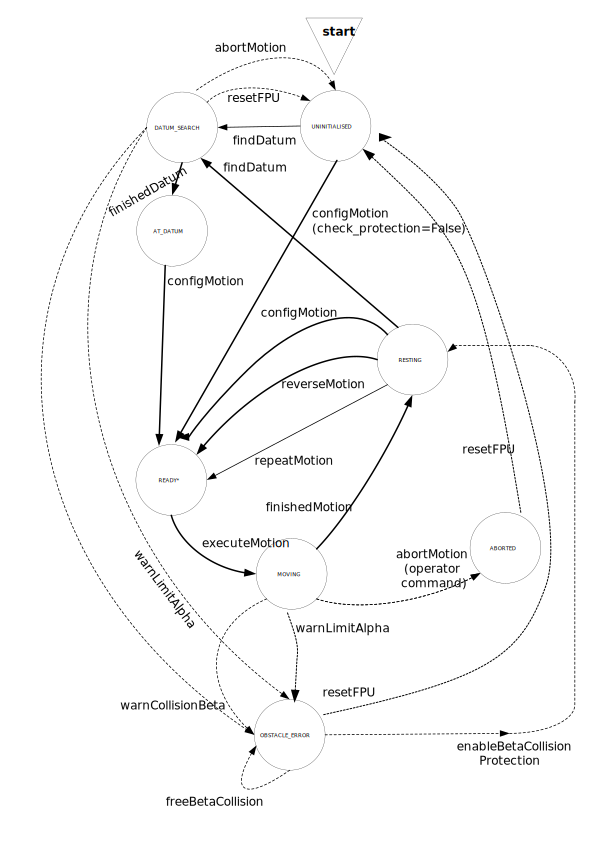
\includegraphics[width=1\textwidth]{FPU-state1.pdf}
  \caption{Allowed state transitions of FPU (CAN protocol version1),
    and the associated driver commands}
  \label{fig:states}
\end{figure}


Figure~\ref{fig:states} on page~\pageref{fig:states} shows, as a
reference, the states of the FPU and commands which are allowed in
protocol version 1.




\section{Common tasks}

The following sections describe several common tasks
and which commands can be used to achieve them.


\subsection{Checking the connection}

At some points, it is of interest what the state of
the connection to the CAN gateway and the FPUs is.
This can be achieved by the following commands:
\begin{minted}{python}
grid_state = gd.getGridState()
grid_state.driver_state  
\end{minted}

The return value is the connection state of the driver, which is
\texttt{DS\_CONNECTED} if the connection is live.  In the case that the
connection fails, it is still possible to retrieve state information
on the FPUs, but it cannot be refreshed any more until the connection
is re-established using the \texttt{connect()} method of the driver
object.

Of course, it is possible that the connection between driver
and EtherCAN gateway works, but that the FPU does not
respond. This can be checked by the commands:

\begin{minted}{python}
  gd.pingFPUs(grid_state)
  grid_state.FPU[0].ping_ok
\end{minted}

In the case that the FPU responds, the returned value is
\texttt{True}.  If the FPU does not respond, the value of the
\verb+ping_ok+ becomes \texttt{False}.



\subsection{Getting the current position}

We already saw how to use the \texttt{pingFPUs()} method
of the driver object. This method automatically
retrieves the current step counters of the FPU.
there are two utility functions which display them:

\begin{minted}{python}
  list_positions(grid_state)
\end{minted}

shows the values of the alpha and beta step counters.
Often, it is interesting to know the value scaled
to an approximate angle. The scaled values
are displayed by the command

\begin{minted}{python}
  list_angles(grid_state)
\end{minted}


One can wonder how this angle is calibrated and what is the relative
position to the datum position. The answer is, these values are not
calibrated - \texttt{list\_angles()} shows only an approximately
scaled value.  Also, the displayed values are only relative to the
datum position, which is defined to have the step counter values
(0,0). If the datum position was not searched at least once before,
both values are meaningless, and \texttt{list\_angles()} returns a
pair of NaN values.




\subsection{Moving the FPU to the datum position}

Because the FPU's step counters need to be zeroed
before any accurate positioning is possible, a
sensible operation early after powering on
the FPU is to move the FPUs to the datum position.
This is done by the command

\begin{minted}{python}
  gd.findDatum(grid_state)
\end{minted}

It is also highly recommend to move the FPUs to the datum position
before powering off. Doing this avoids to have the FPU in an ambiguous
state which might easily lead to hardware damage.

\textbf{Important:} As an important limitation to the CAN protocol
version 1, the \texttt{findDatum()} command mandatory requires that,
before starting the datum search, \textbf{the beta arm is in a
  counter-clockwise position relative to the datum switch}. If the the
step counters have valid values, the beta arm needs to be in a
positive range of valid step counts from the datum switch, or at count
zero. If the beta arm has a position corresponding to the negative
range (that is, clock-wise from the datum position), it needs to be
manually moved first.  This applies also when the step counters in the
meantime have been reset by a \texttt{resetFPU()} command or by
powering off the FPU. You can check whether the step counters are
valid by testing the boolean flag \verb+grid_state.FPU[0].was_zeroed+,
as explained in section~\ref{sec:fpustate} on
page~\pageref{sec:fpustate}.


\subsection{Moving the FPU}

To move the FPU in a precise and safe way, four steps are necessary:

\begin{enumerate}
\item Moving the FPU to the datum position, as explained above.

\item Generating a valid movement waveform table. For a single FPU,
  this is basically a list which defines for a number of short time
  segments how many steps the FPU stepper motors should move, and in
  which direction.

\item Sending the waveform to the FPU
\item Starting the movement
  
\end{enumerate}

There are two options for defining the waveform. The simpler one is to
automatically generate a protocol-conforming waveform where we merely
pass two values which define how much the alpha and beta arms should
move.

\subsubsection{Moving by an angle}

\begin{minted}[linenos]{python}
alpha_move = 45
beta_move = 15

# Generate the required waveform for one FPU
waveform = gen_wf(alpha_move, beta_move)

# upload the waveform to the FPU
gd.configMotion(waveform, grid_state)

# start the movement
print("starting movement by (45,15) degree")
gd.executeMotion(grid_state)
\end{minted}

The above listing shows how to generate a waveform which moves the FPU
by a certain (alpha,beta) angle difference. Note that for CAN protocol
version 1, at least one of alpha and beta must not be zero.

Lines 1 and 2 define variables with the angles we want to move. In
line 5, a new waveform table called \texttt{waveform} is generated
using the \texttt{gen\_wf()} utility function.  By default, this
function generates the quickest valid movement by the angles
requested.

In line 8, the \texttt{configMotion()} method is used to send the
waveform to the FPU. As usual, the \texttt{grid\_state} variable is
passed, and the resulting state of the FPU is returned in this
variable.

Finally, in line 12, the method \texttt{executeMotion()} is called,
which starts the movement of the FPU (or, if we have more than one
FPU, the movement of all of them). In the normal case, this command
blocks and returns when the FPUs have finished moving.  In the case
that there is an error, for example a collision, a Python exception
will be raised.



\subsubsection{Manually defining a waveform table}

\paragraph{Waveform syntax}

In the example above, the waveform was generated by the
\texttt{gen\_wf()} utility function.  For normal movements, this is a
good option, and the actual value of the step counters can always be
retrieved using the \texttt{list\_positions()} utility
function. Sometimes, a much closer control of the FPU movements might
be required. This can be done with a code fragment like this:

\begin{minted}[linenos]{python}
wtable = { 0: [ ( 125, -125),
           ( 140, -140),
           ( 130, -125),
           ( 125, -125),
           ( 10, -20),
           ],
}
gd.configMotion(wtable, grid_state)
\end{minted}

Here, the Python variable wtable is assigned with
a waveform. The required format for a waveform
is \emph{a dictionary with a list of 2-tuples
  with the alpha and beta step counts}. Because
that sounds a bit complex, let's dissect this
structure into its components:

\begin{itemize}
  
\item At the top layer, we have a Python dictionary.  The key of each
  dictionary entry, and integer, is the numerical ID of the FPU we are
  addressing.  Because we only have one FPU, and the numbering starts
  with zero, the key is simply zero.

\item The corresponding value for the key zero is a Python list, as
  indicated by the brackets and a comma-separated sequence. The
  sequence is a list with exactly one entry for each time-slice of the
  movement operation\footnote{With the current default values,
  each time slice has a fixed duration of 250 milliseconds}.

\item Each list entry is a tuple with two elements, both of which are
  numbers. The first element is the number of alpha steps, and the
  second element is the number of beta steps.

  A positive number means that the FPU should move counter-clockwise
  (when viewed from above), and a negative number means it should move
  clock-wise (when viewed from above). If the value is zero, then the
  FPU will rest.

\end{itemize}

Now, we can decipher the above structure into ``in the first time
slice of the movement, the alpha arm should move 125 steps
counter-clockwise, and the beta arm should move 125 steps
clockwise,'' and so on.

\paragraph{Waveform validity rules}

When you define waveforms, they have to conform to a number of rules
and conditions to make sure that the FPU can actually execute
them. These rules are currently as follows:

\begin{enumerate}

\item All step numbers need to be integer values.

\item The first entry needs to have the minimum step count at least
  for one of the two arms.  For protocol version 1, this minimum is fixed to a
  step count of 125\footnote{For protocol version 2, the minimum value
    depends on the duration of a waveform segment which is 250
    milliseconds by default but can be set to another value when
    initializing the driver.}.
  
\item Except the the last non-zero entry, all step numbers in a
  waveform need to have an absolute value which has at least the
  minimum value of 125, and at most the maximum value of 500. Also,
  sequences of zeroes are allowed.

\item A waveform can include several movement parts for each arm. A
  movement part is a sequence of step counts which are non-zero and
  have the same direction. The last entry of a movement part in one
  direction can have a step count between zero and the minimum step
  count. It must not be larger than the minimum step count.

\item When changing the movement direction, the absolute number of
  steps before the change needs to be between zero and the minimum
  step count, followed by a wave table segment with a step count of
  zero, followed by the minimum step count with the opposite sign.

\item The total number of waveform entries can only be 128 (for
  protocol version 1\footnote{In version 2 of the firmware
    communication protocol, this limit is raised to a value of 256}).

\item Between consecutive step number values, the absolute value of
  the larger number can only be at most 40\% larger than the absolute
  value of the smaller number. Also, a change from zero to the minimum
  value, or from a value not larger than the minimum value to zero is
  allowed.

  
\end{enumerate}



\subsection{Aborting a movement}

In the case that one wants to abort a \texttt{findDatum()} or a
\texttt{executeMotion()} operation, one can press
\verb+<Control-c>+. This terminates the movement in about 0.1
seconds. \footnote{Under the hood, this generates a \texttt{SIGINT}
  signal which is during the operation of both commands caught be the
  Python interpreter. The Python interpreter then sends an
  \texttt{abortMotion()} command to the driver object, which results
  in an \texttt{ABORT\_MOTION} CAN message.}

If it is necessary to abort a movement from Python -- for example,
from another Python thread -- this can be done using the
\texttt{abortMotion()} method of the grid driver object.  Like all
driver object methods, this method is thread-safe.

For other driver methods, a \verb+<Control-c>+ normally aborts the
current Python script when the method returns.\footnote{In some cases,
  it can happen that the Python program is stuck on a failed socket
  connection. Terminating such a connection can take considerable time
  because sockets are handled by the Linux kernel and by default, the
  kernel tries extremely hard to keep and re-animate an unreliable
  connection, even if the physical link is temporarily broken. To
  terminate such a hung program, it can be suspended using
  \texttt{<Control-z>} (which sends a SIGSTOP signal) and then
  terminated using the UNIX \texttt{kill} shell command, or using
  \texttt{<Control-\textbackslash>}, which generates a
  \texttt{SIGQUIT} signal.}


\subsection{Reversing a movement}
Often, an FPU has been moved away from the datum position, and it is
desired to move it back to the datum position.  This can be done using
the following method:

\begin{minted}{python}
gd.reverseMotion(grid_state)
\end{minted}

Reversing the waveform requires that there is, firstly, a current
waveform configured, and, secondly, that this waveform remains valid.
After any normal, successful movement, a waveform remains valid for
repetition or reversal. After any collision, limit switch breach, or
abortion of a movement, the waveform becomes invalid. Generally
spoken, a waveform becomes invalid when either, the movement it
describes was interrupted and not completed, or when the step counters
become invalid (for example due to a collision when the FPU is
resting).


\subsection{Repeating a movement}

Sometimes, a waveform for moving in a certain direction has been
configured, and this movement just needs to be repeated.  To do this,
use the following code:

\begin{minted}{python}
gd.repeatMotion(grid_state)
\end{minted}


\section{Recovery from collisions and limit breaches}
\label{sec:recovery}

Because the FPUs are controlled individually, and the CAN-level driver
has absolutely no concept of their geometric configuration, it cannot
take care to move them so that collisions are avoided.  Instead, the
hardware needs to handle collisions in a way that no damage results
and communicate such situations back to the higher layers of the
software.

The following section explains how this is achieved.

\subsection{What happens when a collision or limit switch breach occurs}

Situations in which the movement of the hardware is obstructed
are either collisions between FPUs or limit switch breaches
of the alpha arm. Limit switch breaches are detected
when the alpha arm detects a transition where the
limit switch is on and goes off. All other cases are
considered collisions, which is detected by electrical
circuits which protect the beta arm. This includes
movements where the beta arm is moved out of its
allowed range.

When a collision or limit switch breach occurs, the FPU electronic
hardware stops any movement, and sends a message to the driver. On
receiving such a message, the driver registers the state of the FPU in
the internal \texttt{grid\_state} structure. This is reflected in the
status flags of the FPU, which were discussed above in section
\ref{sec:fpustate} on page \pageref{sec:fpustate}.  The \texttt{state}
field of the FPU is set to the value \texttt{OBSTACLE\_ERROR}, the
flags \texttt{beta\_collision} and \texttt{at\_alpha\_limit} are set
accordingly, and the flag \texttt{was\_zeroed} is cleared.

If any movement operation or \texttt{findDatum()} command is going on,
this command returns with the updated state information on the
collision, and without further waiting for the movement to complete.
When the driver call returns to the Python wrapper, the error is
checked for and transformed into a Python exception. If the exception
is not caught, this terminates the Python script.

It is also possible that a collision occurs while an FPU is \emph{not}
moving and the driver not executing a command.  In this case, the
internal \texttt{grid\_state} structure is changed, too. When the user
tries to launch a new command, the changed state is detected, and if
the command is not valid in collided state, the called method also
raises an exception.\footnote{Because movement methods return on the
  first collision, but in a multi-FPU grid additional collisions can
  occur after that, when controlling multiple FPUs it is a good idea
  to retrieve an updated grid state structure after handling any
  collision.}

The following recipe excludes the task of determining in which
direction FPUs should be moved after a collision.  In the general
case, this can be a complex question. The \texttt{grid\_state}
structure is designed to provide a host of information for making this
decision.

\subsection{Resolution of a beta arm collision}

In case of a collision of a beta arm, there are two special member
functions of the grid driver object for resolving this. The following
snippet shows how to use them:

\begin{minted}[linenos]{python}
  from FpuGridDriver import REQD_CLOCKWISE, REQD_ANTI_CLOCKWISE
  fpu_id = 0
  gd.freeBetaCollision(fpu_id, REQD_CLOCKWISE, grid_state)
  # required for firmware version 1
  gd.pingFPUs(grid_state)
  gd.enableBetaCollisionProtection(grid_state)
\end{minted}

The effect of these lines is as follows:

In line 1, the symbols \texttt{REQD\_CLOCKWISE} and
\texttt{REQD\_ANTI\_CLOCKWISE} are imported.  Then, the parameter
\texttt{fpu\_id} is set to the numerical ID of the FPU, which is zero
for a single-FPU grid. Then, calling the method
\texttt{freeBetaCollision()} moves the collided FPU into the direction
passed in the second parameter - clockwise, or anti-clockwise. When
using the protocol version 1, it is then necessary to retrieve an
update for position and state of the FPU using the \texttt{pingFPUs()}
command.

This might need to be repeated a few times, and verified using visual
inspection, or camera pictures. When the collision is resolved, the
FPU can be switched to the normal state using the
\texttt{enableBetaCollisionProtection()} command.  After this, the FPU
can be moved normally. Because any previously configured waveforms
become invalid, a new movement needs to be configured using
\texttt{configMotion()} at this point. To make movements precise, a
new datum search is required as well.

\subsection{Resolution of an alpha limit switch breach}

For firmware and CAN protocol  version 2, limit switch
breaches can be handled in an analogous way as the
beta arm collisions. For CAN protocol version 1,
is option is not available. Instead, the following
steps are required:

\begin{minted}[linenos]{python}
  # Determine and write down the last movement of the FPU before
  # running into the limit switch. Let's assume
  # the alpha arm was moved with a positive sign.

  # reset the FPU to allow for movements
  gd.resetFPUs(grid_state)

  # move the FPU into the opposite direction
  waveform = gen_wf(-5, 0)
  gd.configMotion(waveform, grid_state, check_protection=False)
  gd.executeMotion(grid_state)
  # A second limit switch breach exception happens here!

  # reset the FPU again, to clear the second breach
  gd.resetFPUs(grid_state)
  gd.configMotion(waveform, grid_state, check_protection=False)
  gd.executeMotion(grid_state)

  gd.findDatum(grid_state)
  
\end{minted}
  

What these operations do is basically to clear the breach state, and
to manually move the FPU.  The flag \texttt{check\_protection=False}
in line 10 is required because normally, the software does not accept
a movement of an FPU which was not zeroed by a datum operation,
and both the limit switch breach and the reset command clear the
\texttt{was\_zeroed} flag.

However, in this state, we \emph{must not} use a datum operation,
therefore it is necessary to override this software protection.

After this, the FPU can be moved, but because it crosses
the limit switch a second time, another limit switch
message is generated, and the FPU needs to be moved
manually for a second time.

\textbf{It is very important that, when resolving such a limit switch
  breach, the FPU is not moved into the same direction as it was
  moving before.  Otherwise, the FPU would run into the hard stop, and
  there is no hardware or software protection which could prevent
  damage in this case}.


\subsection{Limitations of CAN protocol version 1}

The following are the main limitations and functional
differences for protocol version 1:

\begin{itemize}
\item There is no automatic recovery method for alpha
  limit switch breaches. Limit switch breaches need
  to be recovered manually, and it must be carefully
  observed to move the FPU in the correct direction,
  on order to prevent the risk of damage. Especially,
  a datum search must not be used after an alpha limit switch
  breach.

\item The \texttt{findDatum()} method is only allowed if the beta arm
  is at the datum position or in counter-clockwise direction of the
  datum switch.

\item The current position and direction of movement of the FPUs is
  not tracked during ongoing movements, and the driver cannot record
  the last movement direction. This has the effect that the user needs
  to verify manually in which direction the FPU was moving before
  resolving a collision or limit switch breach.

\item In protocol version 2, transitions and allowed commands are
  checked much stricter than in protocol 1.  This results in a
  somewhat reduced flexibility, however the stricter checking also
  allows to make stronger assumptions about the current state, and
  makes it possible to perform automatic recovery of multiple collided
  FPUs.
  
\item In some cases, protocol 1 is not able to
  detect lost messages, so that state information
  might be stale.\footnote{For the case of the \texttt{executeMotion()}
  command, a state update is performed automatically
  if no error has occurred.}

\item It is not possible to lock or unlock FPUs, or otherwise to
  exclude FPUs from movement commands.
  
\item Uploading waveforms might take a longer time, especially if the
  waveform has a large number of steps.
  
\end{itemize}

\section{Outline on management of multiple FPUs}

This section attempts to give a broad overview on how a grid with 1000
FPUs can be managed by higher levels of the instrument software.

The driver software can effortlessly send and receive commands to up
to 1005 FPUs. The only requirement is that the grid driver object is
initialised with that number of FPUs, and the corresponding number of
EtherCAN gateways is connected. When the \texttt{grid\_state} variable
is retrieved, it contains the states of \emph{all} FPUs in the
\verb+grid_state.FPU[]+ sequence. So, in order to know what the state
of FPU number 900 is, we simply have to query
\verb+grid_state.FPU[900]+.

To make managing that number of FPUs easier, there exist a few
additional functions. One feature is that \texttt{grid\_state}
variable has a member named \texttt{Counts}, which summarises the
state of all FPUs. As discussed in section~\ref{sec:fpustate} on
page~\pageref{sec:fpustate}, each FPU has a field with the name
\texttt{state}, which is a enumeration value describing its state. If
the enumeration values are converted to integer indices using
\texttt{int()}, the \texttt{Counts} field contains for each index the
number of FPUs which are in the state defined by that index. For
convenience, \texttt{str(grid\_state)} shows \texttt{Count} as a
dictionary with the state names as keys, and the count numbers as
values. So, the expression
\begin{minted}{python}
  grid_state.Counts[int(FpuGridDriver.FPST_RESTING)]
\end{minted}
returns the number of FPUs in \texttt{RESTING} state.

In addition, there is a function with the name
\texttt{getGridStateSummary(grid\_state)} which maps the different states of the
FPUs to a single value. The idea is simply to define an ordering of
all state enumeration values, for example
\begin{quote}
\begin{verbatim}
  UNINITIALIZED < OBSTACLE_ERROR < ABORTED < DATUM_SEARCH
         < AT_DATUM < READY_FORWARD < MOVING < RESTING
\end{verbatim}
\end{quote}

The return value of the function delivers the \emph{smallest} value in
which at least one FPU is.  That means, if a single FPU is in state
\texttt{UNINITIALZED}, and all other FPUs are in state
\texttt{READY\_FORWARD}, the function would describe the state of the
grid as \texttt{GS\_UNINITIALIZED}. This allows to get quickly an overview
which operations can be done consistently.

All driver methods are thread-safe, so they can be used in a GUI
environment, for example.

In addition, it is possible to inquire the state of the grid and of
course the known positions of all FPUs while movements are happening,
using the \texttt{getGridState()} member function of the grid driver
object. Currently, commands are only processed one at a time - this
restriction does not have purely technical reasons, but simply makes
management less messy. The exception from this is the
\texttt{abortMotion()} method, which can be sent at any time, from any
thread.

Finally, there exists a driver method, \texttt{waitForState()} which
waits either for a time-out to happen, or for a specific state of the
grid to be reached. It always returns the updated grid state.

This makes it easy to perform group operations, while providing full
information on the detailed state of things in cases when, for
example, FPUs have a collision and need to be disentangled guided by
geometric information and a high-level resolution strategy.



\section{Reference}
\subsection{Commands}
\subsection{Errors}
\subsection{State Machine}

\appendix

\section{Dependency requirements and installation}



\subsection{Prerequisites}

\begin{enumerate}
  \item For the C++ driver and static library

    
\begin{itemize}
\item gcc-4.9 (essentially, with support for C++11)
\item Linux-2.6 or newer (requiring support for eventfd)
\item glibc-2.3.2 (epoll support)
\end{itemize}

These should be available on all current Linux systems.

\item For the test code and Python bindings

\begin{itemize}
\item Python-2.7
\item boost-1-66 , which can be downloaded from \url{http://www.boost.org/users/download/}
\item git-2.1 (not mandatory\footnote{Git is used to automatically add a version
  string to the python module. If needed, it can be substituted in the
  makefile, by replacing the definition \texttt{GIT\_VERSION} by a
  suitable constant value.})
\end{itemize}
\end{enumerate}


Note that Python might need to be called with the command name
\texttt{python2} on newer systems.

\subsection{Installation of FPU driver module}

\subsubsection{Installing boost libraries}

Recent Boost libraries are required to build the Python module, which
is needed in the verification system (but not in the final ICS
software).

Please keep in mind that any installed different version of boost
libraries is very likely an essential part of your Linux system, so do
\textbf{not} uninstall older versions from your system!

\begin{itemize}
\item for security, verify boost package signature using gnupg

\item unpack boost package:
  
  \begin{minted}{bash}
    $ tar xzf boost_1_66_0.tar.gz
  \end{minted}    

\item build package:

  \begin{minted}{bash}
    $ cd boost_1_66_0/
    $ ./bootstrap.sh
    $ ./b2
  \end{minted}    

\item install package into /usr/local directory:

  \begin{minted}{bash}
    $ su
    # ./b2 install
  \end{minted}    
\end{itemize}

To make the boost libraries accessible when the
final program is run, you need to add the
command

\begin{verbatim}
export LD_LIBRARY_PATH=$LD_LIBRARY_PATH:/usr/local/lib
\end{verbatim}

to your shell configuration (usually, \verb+$HOME/.bashrc+).

Also, you should add the directory with the boost header files (by
default \verb+/usr/local/include+) to the path configured in the environment
variable \verb+CPLUS_INCLUDE_PATH+, so that gcc can find them when building
the module.

\subsubsection{Installing the python-gevent module}

The Python mock-up gateway uses the gevent
library which is used to serve parallel requests
using asynchronous code. In difference to
Python3's asyncio, it is available both in
Pyhon2 and Python3.

Install it as follows:

  \begin{minted}{bash}
    # pip install gevent
  \end{minted}    

(This command seems to be need to be run as root in order to install
  under \texttt{/usr/local}).



\subsubsection{Building the C++ driver library}

The FPU driver is a static library which becomes included in the
Python module.  Build the FPU driver library as follows:

  \begin{minted}{bash}
    $ cd fpu_driver
    $ make driver
  \end{minted}    

This places the static library libfpudriver.a into
the subdirectory "/lib".

\subsubsection{Building the python module}

Run

  \begin{minted}{bash}
    $ make pyext
  \end{minted}    

This builds the binary extension module \verb+fpu_driver.so+
and places it into the subdirectory \verb+/python+.
In the same subdirectory, there are some test
scripts which can be used to test the module.


\section{Running the test gateway} 

In the sub-directory /testing, the package contains a mock-up test
gateway which responds to messages as specified by the hardware
protocol. To run it, change into a new terminal window and
issue

  \begin{minted}{bash}
    $ cd testing
    $ python2 mock_gateway.py
  \end{minted}    


This test code opens three socket connections on localhost and will
display received messages and commands. It will not necessarily
run with the same speed as the hardware but should match the
hardware protocol faithfully.

[In future,] Use the command line option "--help" to check for additional features,
such as simulating communication failures etc.

In another terminal window, you can run the tests:
  \begin{minted}{bash}
    $ python2 -i test_mock/test_findDatum.py
  \end{minted}    
and so on.






\end{document}
